\chapter{System description}\label{se:system_description}
This section will go into details of the structure of the sewer network for which the further work of this project will be based upon.

As mentioned in section \ref{sec:WWTP_challenges} a steady flow of sewage with a fixed level of contaminants is desired such that an optimal utilization of the wastewater treatment plant can be obtained. An area of interest is Fredericia with a sizable population of approximately 40.000 people and industries where some of the largest consists of a brewery, bottling plant, refinery and a dairy plant \cite{Statistic_Denmark}. All of these industries is placed at the outskirts of the city, meaning that the wastewater discharged into the sewer goes through populated areas creating an uneven flow of wastewater to the WWTP. Two main sewer lines separates the northern and southern part of the city. To limit the scope of the project only the northern main sewer line is considered. This line covers the largest part of the households and the industry located in the city. % This excludes the dairy from the scope of the project as it is located southeast from the wastewater treatment plant. 
In figure \ref{fig:kloakgrid_simplified}, a simplified overview is given of the northern main sewer line in Fredricia. The placement of the sewers shown in \ref{fig:kloakgrid_simplified} is obtained from a Geographically Information System (GIS) map publicly available by the municipal of Fredericia \cite{GIS_kort}. The red and green lines indicate sewers with flows of wastewater only and combined sewers with wastewater and surface runoff, respectively. The populated areas are indicated by two different transparent blue colors, to easier be able to distinguish between the different parts of the sewer network. The red transparent areas indicate small to medium sized industry. 
Only the sewer lines out of or between the separate areas are shown. Furthermore the areas connected by a red line has a separate sewer system for surface runoff, which is lead into various ponds or the sea, minimizing the load on the wastewater treatment plant.
The bottling plant, refinery and the brewery is marked by the purple, brown and black rings, respectively. Several inlets for surface runoff connected directly to the main sewer line exists. %The added disturbance from these inlets is neglected on the assumption that the disturbances from the connected areas will be considerable larger.  



\begin{figure}[H]
\centering
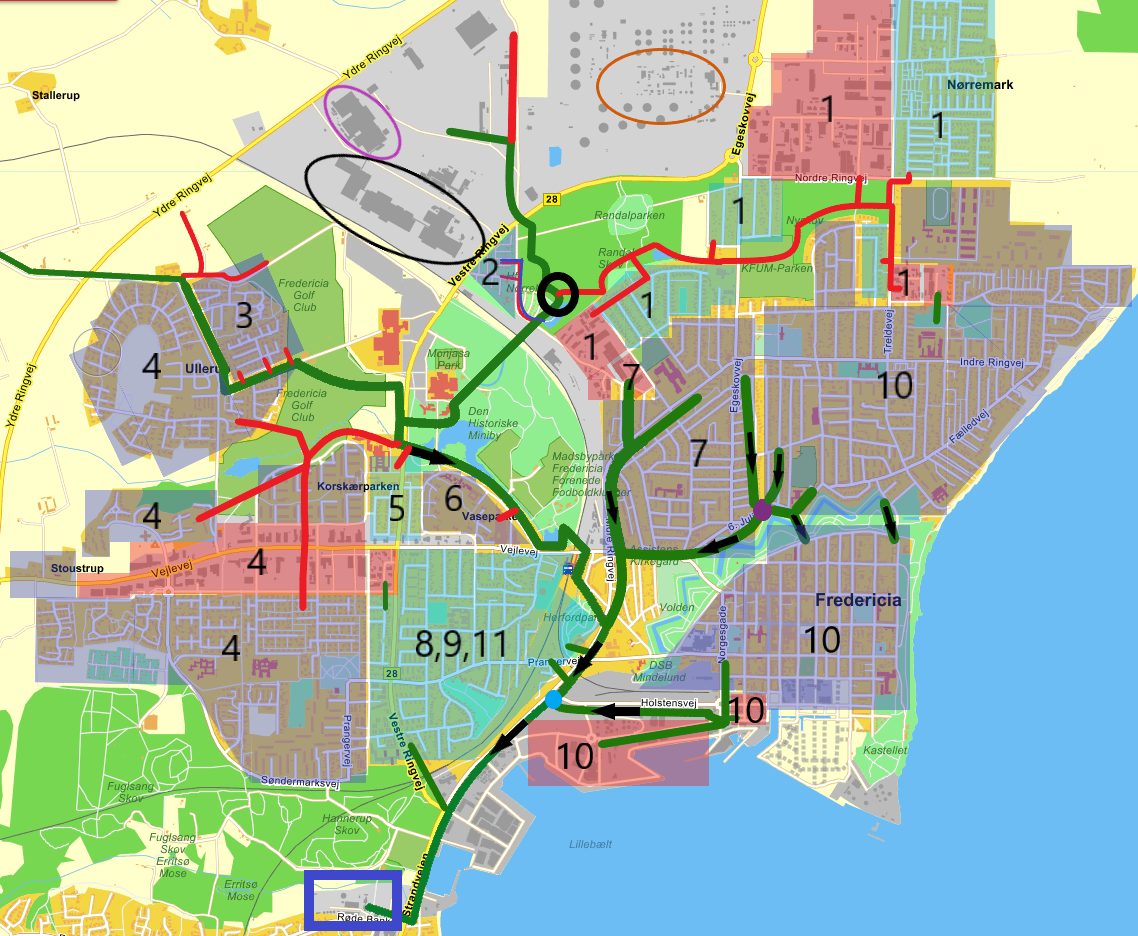
\includegraphics[width=1\textwidth]{report/system_overview/pictures/kloakgrid_simplified9.png}
\caption{Simplified mapping of the northern part of the sewer network in Fredericia. The two blue transparent colors indicate populated areas and the red transparent area indicate industry. Red and green lines is sewers with flows of wastewater and combined wastewater and surface runoff  respectively. Bottling plant, refinery and brewery is marked by purple, brown and black circles respectively. The black circle denotes the start point for the main sewer line. The green sewer line with an yellow line within it is the main sewer line. The purple dot is a connecting point with two incoming and two outgoing sewer lines. Blue dot is a wastewater pumping station which elevates sewage such that gravity can be utilized for the remaining transport into the treatment plant. Blue rectangle marks the location of the wastewater treatment plant.
%Mapping of part of the sewer network in Fredericia. The red and green lines indicate sewers where the red sewers has flows of sewage only and the green line is combined sewage and runoff from urban surfaces. Transparent parts indicate that the area has a connected sewer grid within and the red/green lines from this grid indicates the output from this area. Two shades of transparent blue is used to illustrate sewer systems in populated areas. The red transparent areas indicate minor industry and the black, brown and purple rings is brewery, refinery and bottling plant respectively. The purple dot indicate a splitting point with two incoming and outgoing sewer pipes. The light blue dot is a sewer reservoir before wastewater is led to the wastewater treatment plant indicated by the blue rectangle.
\cite{Krak} \cite{GIS_kort}}
\label{fig:kloakgrid_simplified}
\end{figure}


The various enumerated parts in figure \ref{fig:kloakgrid_simplified} is shown by order of attachment to the main sewer line, together with distance between each attachment, in figure \ref{fig:sewer_line_diagram}. 

\begin{figure}[H]
\centering
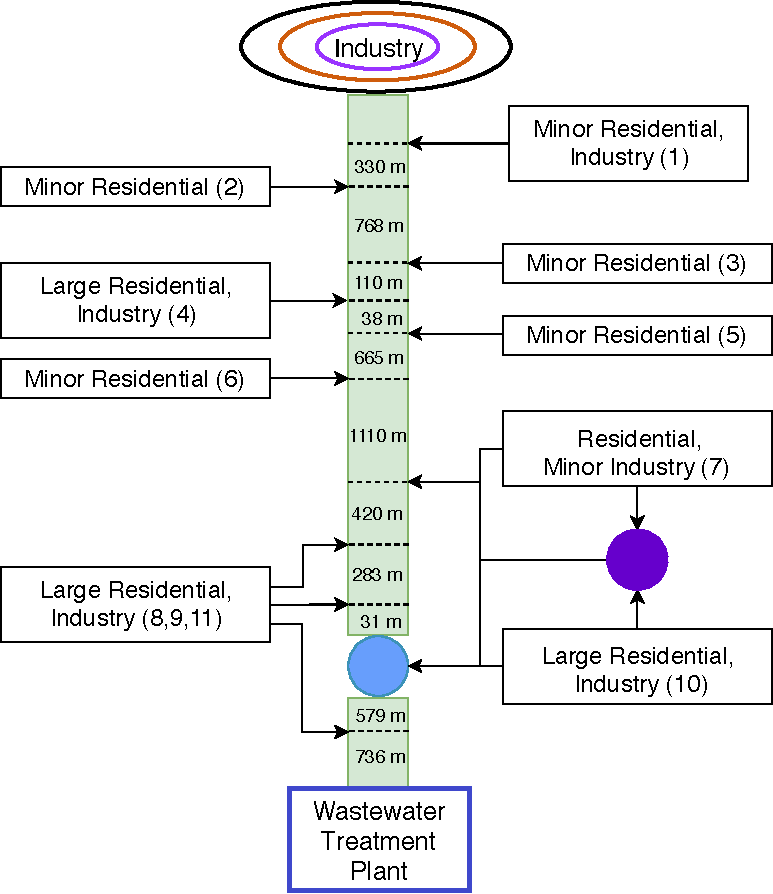
\includegraphics[width=0.6 \textwidth]{report/system_overview/pictures/sewer_line_diagram.pdf}
\caption{Simplification of the attachments to the main sewer line shown in figure \ref{fig:kloakgrid_simplified}. The numbers correspond to which area is connected to the main sewer line farthest from the wastewater treatment plant, with the distance between them \cite{GIS_kort}.}
\label{fig:sewer_line_diagram}
\end{figure}

Furthermore the different sections consist of pipe of varying diameters as can be seen in table \ref{tab:kloak_diameter}.

% \begin{table} 
% \centering
% \begin{tabular}[H]{|c|c|c|} \hline
% %\begin{table}[H]

% \multirow{2}{*}{Pipe section} & Pipe length & Inner pipe diameter \\ 
% 							  & (meter)		& (millimeter)		\\ \hline
% \multirow{2}{*}{1 $\rightarrow$ 2}		  & 303			  & 900	\\
% 						 & 27			  & 1000 \\ \hline
% 						 & 155			  & 1000 \\
% 2 $\rightarrow$ 3		 & 295			  & 800  \\
% 			 			 & 318			  & 900 \\ \hline
% 3 $\rightarrow$ 4		 & 110			  & 900 \\ \hline
% 4 $\rightarrow$ 5		 & 38 			  & 1000 \\ \hline
% 5 $\rightarrow$ 6		 & 665			  & 1000 \\ \hline
% \multirow{2}{*}{6 $\rightarrow$ 7}		 & 155			  & 1000 \\
% 			 			 & 955			  & 1200 \\ \hline
%  						 & 293			  & 1200 \\
% 7 $\rightarrow$ 8		 & 11 			  & 1300 \\
% 			 			 & 116			  & 1200 \\ \hline
% 8 $\rightarrow$ 9		 & 283			  & 1400 \\ \hline
% 9 $\rightarrow$ 10		 & 31			  & 1400 \\ \hline
% 						 & 125			  & 1600 \\
% 10 $\rightarrow$ 11	 	 & 94			  & 1500 \\
% 						 & 360 			  & 1600 \\ \hline
% 11 $\rightarrow$ WWTP    & 736			  & 1600 \\ \hline
% Total length 		     & \multirow{2}{*}{5070}  &		 \\ 
% 1 $\rightarrow$ WWTP     &						  & \\ \hline

% \end{tabular}

% \caption{Table of the various lengths and the approximate inner diameter of pipe, appearing in order, in the main sewer line. Pipe section indicate the length of pipe between the attachment of the various areas to the main sewer line.} 
% \label{tab:kloak_diameter}
% \end{table}


\begin{table} [H]
\centering
\begin{tabular}{|c|c|c|c|c|c|} 
\hline
\rowcolor[HTML]{9B9B9B} 
\multicolumn{1}{|c|}{\cellcolor[HTML]{9B9B9B}\textbf{Pipe section}} & \multicolumn{1}{c|}{\cellcolor[HTML]{9B9B9B}\textbf{\begin{tabular}[c]{@{}c@{}}Pipe length\\ (meter)\end{tabular}}} & \multicolumn{1}{c|}{\cellcolor[HTML]{9B9B9B}\textbf{\begin{tabular}[c]{@{}c@{}}Inner pipe\\ diameter (mm)\end{tabular}}} &
\multicolumn{1}{c|}{\cellcolor[HTML]{9B9B9B}\textbf{\begin{tabular}[c]{@{}c@{}}Bed datum\\ in (m)\end{tabular}}} & \multicolumn{1}{c|}{\cellcolor[HTML]{9B9B9B}\textbf{\begin{tabular}[c]{@{}c@{}}Bed datum\\ out (m)\end{tabular}}} & \multicolumn{1}{c|}{\cellcolor[HTML]{9B9B9B}\textbf{\begin{tabular}[c]{@{}c@{}}Bed\\ slope (\textperthousand)\end{tabular}}} \\ \hline
\multirow{2}{*}{1 $\rightarrow$ 2}		  & 303			  & 900    & 11,56  & 10,65 & 3,00\\
										 & 27			  & 1000   & 10,65  & 10,57 & 3,00 \\ \hline
										 & 155			  & 1000   & 10,57  & 9,94  & 4,10 \\
2 $\rightarrow$ 3						 & 295			  & 800    & 9,94   & 6,33  & 12,20 \\
			 							 & 318			  & 900    & 6,33   & 4,71  & 5,30 \\ \hline
3 $\rightarrow$ 4						 & 110			  & 900    & 4,71   & 4,31  & 3,60 \\ \hline
4 $\rightarrow$ 5						 & 38 			  & 1000   & 4,31   & 4,40  & -2,40 \\ \hline
5 $\rightarrow$ 6						 & 665			  & 1000   & 4,40   & 2,43  & 3,00 \\ \hline
\multirow{2}{*}{6 $\rightarrow$ 7}		 & 155			  & 1000   & 2,43   & 2,31  & 0,80 \\
			 							 & 955			  & 1200   & 2,31   & -0,48&  2,90 \\ \hline
 										 & 293			  & 1200   & -0,48  & unknown&  \\
7 $\rightarrow$ 8						 & 11 			  & 1300   & unknown& -1,38&  \\
			 							 & 116			  & 1200   & -1,38  & -1,62&  2,10\\ \hline
8 $\rightarrow$ 9						 & 283			  & 1400   & -1,62  & -2,09&  1,70\\ \hline
9 $\rightarrow$ 10						 & 31			  & 1400   & -2,09  & -2,15& 1,90 \\ \hline
										 & 125			  & 1600   & 0,31   & 0,05 & 2,10 \\
10 $\rightarrow$ 11	 	 				 & 94			  & 1500   & 0,05   & -0,07& 1,30\\
						 			 	 & 360 			  & 1600   & -0,07  & -1,72& 4,60 \\ \hline
11 $\rightarrow$ WWTP   				 & 736			  & 1600   & -1,72  & -2,60& 1,20\\ \hline
Total length 		    				 & \multirow{2}{*}{5070}  &	  & & & 	 \\ 
1 $\rightarrow$ WWTP    				 &						  &   & & & \\ \hline

\end{tabular}

\caption{Table of the various lengths and the approximate inner diameter of pipe, appearing in order, in the main sewer line. Pipe section indicate the length of pipe between the attachment of the various areas to the main sewer line \cite{GIS_kort}.} 
\label{tab:kloak_diameter}
\end{table}

Some assumptions is made to avoid complications during simulation. The negative slope of the section between connection point four and five is flipped such that no permanent storage of sewage happens. The reason for this assumption is that it will ease the computation, of the free flow in that section, if storage in the pipe sections could be disregarded during simulation. Furthermore the new slope is deemed acceptable based on the obtained slopes for the remaining pipe sections. 
For the two pipe sections between point seven and eight, where out- and input datum is unknown, are gathered in to a single pipe section. This section will be designated an inner diameter of 1200 mm as the section with the larger diameter is assumed insignificant for the free flow at the end points of the entire section.

\begin{table} [H]
\centering
\begin{tabular}{|c|c|c|c|} 
\hline
\rowcolor[HTML]{9B9B9B} 
\multicolumn{1}{|c|}{\cellcolor[HTML]{9B9B9B}\textbf{Pipe section}} & 
\multicolumn{1}{c|}{\cellcolor[HTML]{9B9B9B}\textbf{\begin{tabular}[c]{@{}c@{}}Pipe length\\ (meter)\end{tabular}}} & 
\multicolumn{1}{c|}{\cellcolor[HTML]{9B9B9B}\textbf{\begin{tabular}[c]{@{}c@{}}Inner pipe\\ diameter (mm)\end{tabular}}} &
\multicolumn{1}{c|}{\cellcolor[HTML]{9B9B9B}\textbf{\begin{tabular}[c]{@{}c@{}}Bed\\ slope (\textperthousand)\end{tabular}}} \\ \hline

4 $\rightarrow$ 5						& 38 			  & 1000   & 2,40 \\ \hline

\multirow{2}{*}{7 $\rightarrow$ 8}	 	& 304 			  & 1200   & 3.00  \\
			 							& 116			  & 1200   &   2,10\\ \hline

\end{tabular}
\caption{New slope values for sections with negative slope and unknown values.}
\label{tab:new_slope_values}
\end{table}


To simulate how the wastewater propagation throughout the sewer network the flows in each residential and industrial area needs to be known. However Fredericia does not have measurement of the flow from each area, they only have measurements at some pumping stations across the city. Therefore it is chosen to use the flow profile shown in figure \ref{fig:input_to_wwtp} for the residential areas, as an estimate of the flow across a day. This flow profile will be scaled to fit each residential area in figure \ref{fig:sewer_line_diagram}.

From figure \ref{fig:kloakgrid_simplified} it can be seen that 11 different flow profiles needs to constructed to cover each residential and industrial area. Each of these residential and industrial areas have been measured to give an estimate of the area for each zone. In table \ref{tab:size_of_areas} the size of the residential and industrial areas are shown. 

\begin{table}[H]
\centering
\begin{tabular}{|c|c|c|}
\hline
\textbf{Zone} & \textbf{\begin{tabular}[c]{@{}c@{}}Residential\\ area\\ $[km^2]$\end{tabular}} & \textbf{\begin{tabular}[c]{@{}c@{}}Industrial\\ area\\ $[km^2]$\end{tabular}} \\ \hline
1 - Thulesvej & 0,167                                                                        & 0,0083                                                                      \\ \hline
1 - Nørremark & 0,458                                                                        & 0,543                                                                       \\ \hline
2             & 0,056                                                                        & -                                                                           \\ \hline
3             & 0,167                                                                        & -                                                                           \\ \hline
4             & 1,872                                                                        & 0,375                                                                       \\ \hline
5             & 0,104                                                                        & -                                                                           \\ \hline
6             & 0,115                                                                        & -                                                                           \\ \hline
7             & 0,771                                                                        & 0,014                                                                       \\ \hline
8-9           & 0,667                                                                        & 0,021                                                                       \\ \hline
10            & -                                                                            & -                                                                           \\ \hline
11            & 0,278                                                                        & -                                                                           \\ \hline
\end{tabular}
\caption{Table over the size of the are different residential and industrial zones.}
\label{tab:size_of_areas}
\end{table}

By knowing the area and assuming that the density of the population is the same across the city, hence a flow profile can be scale to each of the residential and industrial areas. In figure \ref{fig:flow_profile_thulevej} a flow profile is shown for Thulesvej which is located in residential area one closet to the main sewer line. 

%Furthermore, from one of the pumping stations a measurement is obtained that illustrates the flow from that zone. This will be used to construct a flow profile according to the area that this pumping station is covering. 

\begin{figure}[H]
\centering
% This file was created by matlab2tikz.
%
%The latest updates can be retrieved from
%  http://www.mathworks.com/matlabcentral/fileexchange/22022-matlab2tikz-matlab2tikz
%where you can also make suggestions and rate matlab2tikz.
%
\definecolor{mycolor1}{rgb}{0.00000,0.44700,0.74100}%
%
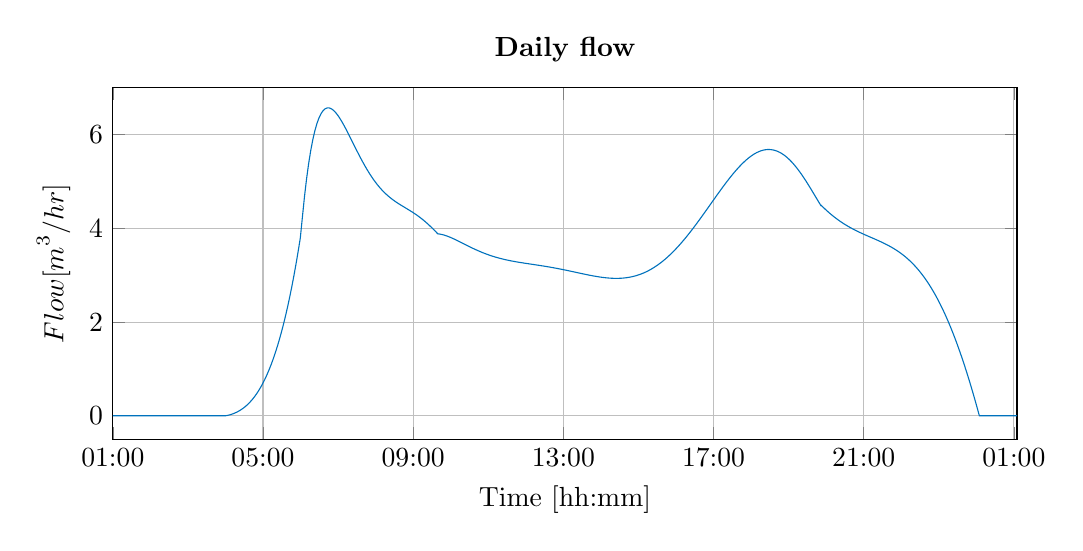
\begin{tikzpicture}

\begin{axis}[%
width=4.521in,
height=1.7566in,
at={(0.758in,0.481in)},
scale only axis,
xmin=3600,
xmax=90000,
scaled x ticks = false,
xtick={3600,17950,32300,46650,61000,75350,89700},
xticklabels={{01:00},{05:00},{09:00},{13:00},{17:00},{21:00},{01:00},{},{},{}},
xlabel={Time [hh:mm]},
xmajorgrids,
ymin=-0.5,
ymax=7,
ylabel={$\text{Flow [m}^\text{3}\text{/hr]}$},
ymajorgrids,
axis background/.style={fill=white},
title style={font=\bfseries},
title={Daily flow},
legend style={legend cell align=left,align=left,draw=white!15!black}
]
\addplot [color=mycolor1,solid]
  table[row sep=crcr]{%
3599	0\\
3799	0\\
3998	0\\
4197	0\\
4396	0\\
4595	0\\
4794	0\\
4993	0\\
5192	0\\
5391	0\\
5590	0\\
5789	0\\
5988	0\\
6188	0\\
6387	0\\
6586	0\\
6785	0\\
6984	0\\
7183	0\\
7382	0\\
7581	0\\
7780	0\\
7979	0\\
8178	0\\
8377	0\\
8577	0\\
8776	0\\
8975	0\\
9174	0\\
9373	0\\
9572	0\\
9771	0\\
9970	0\\
10169	0\\
10368	0\\
10567	0\\
10766	0\\
10965	0\\
11165	0\\
11364	0\\
11563	0\\
11762	0\\
11961	0\\
12160	0\\
12359	0\\
12558	0\\
12757	0\\
12956	0\\
13155	0\\
13354	0\\
13554	0\\
13753	0\\
13952	0\\
14151	0\\
14350	0\\
14549	0.00710028180255936\\
14748	0.0184228250217605\\
14947	0.0320492223793003\\
15146	0.0482073693016751\\
15345	0.0671355323234623\\
15544	0.0890823640800493\\
15743	0.114306906530896\\
15942	0.143078582413403\\
16142	0.175851135929245\\
16341	0.212588195200944\\
16540	0.253744214191448\\
16739	0.299629869141819\\
16938	0.350565997430973\\
17137	0.406883518354036\\
17336	0.468923342131185\\
17535	0.537036267147258\\
17734	0.611582865421718\\
17933	0.692933356309431\\
18132	0.781467468431938\\
18331	0.877574289839258\\
18531	0.982195922443594\\
18730	1.09469519004965\\
18929	1.21599102593738\\
19128	1.3465082650137\\
19327	1.48668017480407\\
19526	1.63694823493869\\
19725	1.79776190486959\\
19924	1.96957837981796\\
20123	2.15286233495235\\
20322	2.34808565779734\\
20521	2.55572716887281\\
20720	2.77627233056388\\
20920	3.0114231889665\\
21119	3.25932816256334\\
21318	3.52163248137147\\
21517	3.79884505460662\\
21716	4.24535835961483\\
21915	4.68162393830136\\
22114	5.0605303399952\\
22313	5.38652724971494\\
22512	5.66385308888405\\
22711	5.89653976849929\\
22910	6.08841744227553\\
23109	6.24311925981753\\
23308	6.36408611977997\\
23508	6.45495440917018\\
23707	6.51789852026043\\
23906	6.55633849014062\\
24105	6.57299288668956\\
24175	6.57415203876262\\
24304	6.57041181650709\\
24503	6.55098167809271\\
24702	6.51692991498017\\
24901	6.4703297689161\\
25100	6.41310503299458\\
25299	6.3470348048595\\
25498	6.2737582398154\\
25697	6.19477930401627\\
25897	6.11104412197444\\
26096	6.02464281487946\\
26295	5.93629279768905\\
26494	5.84700423972142\\
26693	5.75767591081538\\
26892	5.66909993449537\\
27091	5.58196654112981\\
27290	5.4968688210775\\
27489	5.41430747787304\\
27688	5.33469558136816\\
27887	5.25836332089683\\
28086	5.18556275841323\\
28285	5.11647258168728\\
28485	5.0508846198317\\
28684	4.98950099222484\\
28883	4.93197089391124\\
29082	4.87822678626446\\
29281	4.82815154614999\\
29480	4.78158321907345\\
29679	4.73831977233886\\
29878	4.69812384820355\\
30077	4.66072751704663\\
30276	4.62583703052387\\
30475	4.59313757473281\\
30674	4.5622980233338\\
30874	4.53283158549684\\
31073	4.50468196016016\\
31272	4.4773467537562\\
31471	4.45047714751611\\
31670	4.42373179994733\\
31869	4.39678159999861\\
32068	4.36931442022513\\
32267	4.34103986992983\\
32466	4.31169404831157\\
32665	4.28104429767759\\
32864	4.24889395655103\\
33063	4.21508711284956\\
33263	4.17933000884771\\
33462	4.14191994481735\\
33661	4.1026777909942\\
33860	4.06165847677637\\
34059	4.01898147061914\\
34258	3.97483553325084\\
34457	3.92948347075326\\
34656	3.88397722505031\\
34855	3.87828619696292\\
35054	3.86930343292533\\
35253	3.85747628069986\\
35452	3.84321750420727\\
35651	3.8269069276083\\
35851	3.80879876200495\\
36050	3.78939405265094\\
36249	3.76889654705036\\
36448	3.74756974114895\\
36647	3.72565176386635\\
36846	3.70335676254554\\
37045	3.68087624735635\\
37244	3.65838039499861\\
37443	3.63601931223958\\
37642	3.61392425970557\\
37841	3.59220883690962\\
38040	3.57097012832554\\
38240	3.55018741982724\\
38439	3.53013612801473\\
38638	3.51076484830304\\
38837	3.49211525526681\\
39036	3.47421768422563\\
39235	3.45709205706402\\
39434	3.44074877307242\\
39633	3.42518956535756\\
39832	3.41040832363483\\
40031	3.39639188339584\\
40230	3.38312078275112\\
40429	3.37056998660284\\
40628	3.35870957943378\\
40828	3.34745071919719\\
41027	3.33686810559657\\
41226	3.32686310213515\\
41425	3.31739257121347\\
41624	3.30841150350928\\
41823	3.29987353111825\\
42022	3.29173141295388\\
42221	3.28393749256906\\
42420	3.27644412877175\\
42619	3.26920410036191\\
42818	3.26217098429212\\
43017	3.25529950899909\\
43217	3.24851217065511\\
43416	3.24183466319726\\
43615	3.23519285663449\\
43814	3.22854913912451\\
44013	3.22186845469703\\
44212	3.21511851496282\\
44411	3.20826998920971\\
44610	3.20129667325793\\
44809	3.19417563788733\\
45008	3.18688735701933\\
45207	3.17941581621549\\
45406	3.17174860242722\\
45606	3.16383689263074\\
45805	3.15575477699682\\
46004	3.14746198091052\\
46203	3.13896104857063\\
46402	3.13025830584381\\
46601	3.12136384673614\\
46800	3.11229150416268\\
46999	3.10305880603746\\
47198	3.09368691713768\\
47397	3.08420056695858\\
47596	3.07462796451394\\
47795	3.06500070041369\\
47994	3.05535363674715\\
48194	3.04567651271804\\
48393	3.03610730717207\\
48592	3.02664147037229\\
48791	3.01732563630324\\
48990	3.0082089940022\\
49189	2.99934311547402\\
49388	2.99078177508811\\
49587	2.98258076072152\\
49786	2.97479767731173\\
49985	2.96749174408537\\
50184	2.96072358490748\\
50383	2.95455501286881\\
50583	2.94902291968129\\
50782	2.94424641889452\\
50981	2.94026017220989\\
51180	2.93712849821384\\
51379	2.93491575689753\\
51578	2.9336861111075\\
51712	2.93344399692937\\
51777	2.93350328374416\\
51976	2.93443031534624\\
52175	2.9365293193663\\
52374	2.93986123720252\\
52573	2.94448559316272\\
52772	2.95046024994984\\
52971	2.95784116492597\\
53171	2.96673035011726\\
53370	2.97709054566539\\
53569	2.98901126884894\\
53768	3.00253844381405\\
53967	3.01771490395241\\
54166	3.03458016521482\\
54365	3.0531702045435\\
54564	3.07351724286139\\
54763	3.09564953469017\\
54962	3.11959116348308\\
55161	3.14536184343757\\
55360	3.17297672953474\\
55560	3.2025990174384\\
55759	3.23393799133826\\
55958	3.26713748554458\\
56157	3.30219265112997\\
56356	3.33909325560095\\
56555	3.37782354681432\\
56754	3.41836212902034\\
56953	3.46068185036243\\
57152	3.50474970132568\\
57351	3.55052672761426\\
57550	3.59796795453961\\
57749	3.64702232576993\\
57949	3.69789080473406\\
58148	3.75000107940876\\
58347	3.80353407849953\\
58546	3.85841406720561\\
58745	3.91455914615849\\
58944	3.97188128289352\\
59143	4.03028636135278\\
59342	4.08967424906017\\
59541	4.14993888181998\\
59740	4.21096836895186\\
59939	4.27264511666528\\
60138	4.33484597199087\\
60337	4.39744238646266\\
60537	4.460616902581\\
60736	4.52359842141341\\
60935	4.58655871601919\\
61134	4.64934970900322\\
61333	4.7118190777594\\
61532	4.77381055242879\\
61731	4.83516423899175\\
61930	4.89571696741947\\
62129	4.95530266351737\\
62328	5.01375274828578\\
62527	5.07089656280736\\
62726	5.12656181990029\\
62926	5.1808420410537\\
63125	5.23301961581908\\
63324	5.28319605858069\\
63523	5.33119764669666\\
63722	5.37685171215669\\
63921	5.41998726577409\\
64120	5.46043565259203\\
64319	5.49803123715681\\
64518	5.53261212032364\\
64717	5.56402088975496\\
64916	5.5921054013216\\
65115	5.61671959434555\\
65314	5.63772434100905\\
65514	5.65506542608248\\
65713	5.66844637033604\\
65912	5.67785054580365\\
66111	5.68317579333198\\
66265	5.6844393264031\\
66310	5.68433166094568\\
66509	5.68124046587969\\
66708	5.67383839505733\\
66907	5.66207664129223\\
67106	5.64592258155172\\
67305	5.62536099087637\\
67504	5.60039529730472\\
67703	5.57104887762718\\
67903	5.5371862865325\\
68102	5.49921381139279\\
68301	5.45706450861086\\
68500	5.41085544542991\\
68699	5.36073073781378\\
68898	5.30686309653841\\
69097	5.24945541691582\\
69296	5.18874241446603\\
69495	5.12499230152653\\
69694	5.05850851408906\\
69893	4.9896314807656\\
70092	4.91874043928682\\
70292	4.84588779072665\\
70491	4.77226660569418\\
70690	4.6980235194415\\
70889	4.62371235792628\\
71088	4.54993556513772\\
71260	4.48710030274668\\
71287	4.49353726057994\\
71486	4.44947345408763\\
71685	4.407048692502\\
71884	4.36625858371511\\
72083	4.32709083435589\\
72282	4.289525499708\\
72481	4.25353523389844\\
72680	4.21908554009987\\
72880	4.18597314726358\\
73079	4.15448091308838\\
73278	4.12438506605859\\
73477	4.09562497625584\\
73676	4.06813411464458\\
73875	4.04184030327419\\
74074	4.01666596530525\\
74273	3.99252837517106\\
74472	3.96933990887471\\
74671	3.94700829381207\\
74870	3.92543685921783\\
75069	3.9045247860968\\
75269	3.88406627795044\\
75468	3.86415709197283\\
75667	3.84458185304801\\
75866	3.82522563565619\\
76065	3.80597061808801\\
76264	3.78669633247073\\
76463	3.76727991501112\\
76662	3.74759635595384\\
76861	3.72751874991917\\
77060	3.70691854598326\\
77259	3.68566579766375\\
77458	3.66362941327093\\
77657	3.64067740596097\\
77857	3.61655366789701\\
78056	3.5913658514955\\
78255	3.56486291252174\\
78454	3.53691178579501\\
78653	3.50737976303432\\
78852	3.4761347426544\\
79051	3.44304548025224\\
79250	3.40798183840312\\
79449	3.37081503706588\\
79648	3.33141790363627\\
79847	3.28966512291887\\
80046	3.24543348750541\\
80246	3.19836004897266\\
80445	3.14879681142805\\
80644	3.09639967201374\\
80843	3.04105637174048\\
81042	2.98265801102665\\
81241	2.92109930000879\\
81440	2.85627880878449\\
81639	2.78809921741142\\
81838	2.71646756609606\\
82037	2.64129550526046\\
82236	2.56249954575803\\
82435	2.4800013090622\\
82635	2.39328459231101\\
82834	2.30314888751374\\
83033	2.20910864015839\\
83232	2.11110844635167\\
83431	2.0090992647929\\
83630	1.90303866671892\\
83829	1.79289108603862\\
84028	1.67862806962992\\
84227	1.56022852735244\\
84426	1.43767898193824\\
84625	1.31097381977632\\
84824	1.1801155402888\\
85023	1.04511500664776\\
85223	0.905282216762484\\
85422	0.762043980613217\\
85621	0.614748973653748\\
85820	0.463444062107368\\
86019	0.308185727662584\\
86218	0.149040317526378\\
86401	0\\
86417	0\\
86616	0\\
86815	0\\
87014	0\\
87213	0\\
87412	0\\
87612	0\\
87811	0\\
88010	0\\
88209	0\\
88408	0\\
88607	0\\
88806	0\\
89005	0\\
89204	0\\
89403	0\\
89602	0\\
90000	0\\
};
%\addlegendentry{Zone 1,1};

\end{axis}
\end{tikzpicture}%
\caption{A flow profile for Thulesvej.}
\label{fig:flow_profile_thulevej}
\end{figure}  \fxnote{skal tilpasse thulesvej, samt enheden skal selvfølgelig være m3/s}

From the data given by Fredericia WWTP, which can be seen in attachments /Data\_pump\_stations/Thulesvej-217, this flow profile have been constructed to fit a working day flow for Thulesvej. It has been chosen to only produce flow profiles for working days and therefore non of the profiles fits a weekend. This profile covers both the wastewater from the residential and industrial area at Thulesvej. The remaining flow profiles for the rest of the zones can be seen in appendix \fxnote{appendix mangler, samt en reference}. Furthermore, these flow profiles illustrates the input flow into the main sewer line, and therefore some of the flow profiles will have added a delay, due to longer transport time from the zone to the main sewer line. An explanation for each profile to a zone is given below.    

The residential areas denoted with one in figure \ref{fig:sewer_line_diagram}, stretch across a long sewer line. Where the sewage have to be transported a longer distance from the zone furthest away before reaching the main sewer line. It is therefore chosen to make two flow profiles, one from the residential and industrial area right next to the main sewer line, and one for the rest of the zones. These two flow profiles will be add together, and thereby the peaks will be extended for a longer period than a normal profile. The industrial area consists mainly of auto shops, recycle factory and workshops and therefore they will have the same flow profile as for residential area. 

From the second zone only one flow profile will be used and as the zone is close to main sewer line no delay in the profile is added. At zone three the distance from the residential area to the main sewer line is long, and therefore a delay will be added. The fourth zone covers a larger area and as some of the residential are far away from the main sewer line, therefore the flow profile is extended in the peaks. The industrial consists of grocery stores, workshops and car shops and therefore will have the same flow profile.

Zone five and six will have a normal profiles without delays. Zone seven will have a profile with delay as it also stretch across a long sewer line before reaching the main sewer line. Zone eight, nine and eleven will all have the same profile just scaled according to the size of the zones, and the industrial area is the same as the one in zone four. 

From zone ten a pump is pumping the wastewater to the main sewer line every 30 minuted for a period of 15 minutes. The pump has a pumping capacity of 0,350 $m^3/s$ which have been state by Fredericia. Therefore the flow profile for this area will be a constant input of 0,350 $m^3/s$ for 15 minutes every 30 minute.     